\documentclass[10pt]{report}
\usepackage[utf8]{inputenc}
\usepackage[italian]{babel}
\usepackage{multicol}
\usepackage[bookmarks]{hyperref}
\usepackage[a4paper, total={18cm, 25cm}]{geometry}
\usepackage{graphicx}
\usepackage{xcolor}
\usepackage{textcomp}
\graphicspath{ {./img/} }
\usepackage{listings}
\usepackage{makecell}
\usepackage{qtree}
\usepackage{pgfplots}
\usepackage{tikz}
\usepgflibrary{shapes}
\usepgfplotslibrary{fillbetween}
\definecolor{backcolour}{RGB}{255,255,255}
\definecolor{codegreen}{RGB}{27,168,11}
\definecolor{codeblue}{RGB}{35,35,205}
\definecolor{codegray}{RGB}{128,128,128}
\definecolor{codepurple}{RGB}{205,35,56}
\lstdefinestyle{myPython}{
	backgroundcolor=\color{backcolour},   
	commentstyle=\color{codegreen},
	keywordstyle=\color{codeblue},
	numberstyle=\tiny\color{codegray},
	stringstyle=\color{codepurple},
	basicstyle=\small\ttfamily,
	breakatwhitespace=false,         
	breaklines=true,                 
	captionpos=b,                    
	keepspaces=true,                 
	numbers=left,                    
	numbersep=2pt,                  
	showspaces=false,                
	showstringspaces=false,
	showtabs=false,                  
	tabsize=2,
	language=python
}
\lstdefinestyle{myC}{
	backgroundcolor=\color{backcolour},   
	commentstyle=\color{codegreen},
	keywordstyle=\color{codeblue},
	numberstyle=\tiny\color{codegray},
	stringstyle=\color{codepurple},
	basicstyle=\small\ttfamily,
	breakatwhitespace=false,         
	breaklines=true,                 
	captionpos=b,                    
	keepspaces=true,                 
	numbers=left,                    
	numbersep=2pt,                  
	showspaces=false,                
	showstringspaces=false,
	showtabs=false,                  
	tabsize=2,
	language=C
}
\newcommand*\triangled[1]{\tikz[baseline=(char.base)]{
            \node[regular polygon, regular polygon sides=3,draw,inner sep=1pt] (char) {#1};}}
            
\usepackage{fancyhdr}
\pagestyle{fancy}
\renewcommand{\headrulewidth}{0pt}
\fancyhead{}
\fancyfoot[L]{Telegram: \texttt{@fexed}}
\fancyfoot[R]{Github: \texttt{fexed}}
\begin{document}
\title{Parallel and Distributed Systems}
\author{Federico Matteoni}
\date{A.A. 2021/22}
\renewcommand*\contentsname{Index}

\maketitle
\tableofcontents
\pagebreak
\section{Introduction}
Prof.: Marco Danelutto
\paragraph{Program} Techniques for both parallel (single system, many core) and distributed (clusters of systems) systems.\\
Principles of parallel programming, structured parallel programming, parallel programming lab with standard and advanced (general purpose) \textbf{parallel programming frameworks}.
\paragraph{Technical Introduction} Each machine has more cores, perhaps multithreaded cores, but also GPUs (maybe with AVX support, which support operations floating point operations, \textbf{flops}, in a single instruction).\\
Between 1950 and 2000 the VLSI technology arised, integrated circuits which nowadays are in the order of 7nm (moving towards 2nm): printed circuits!\\
In origin, everything happened in a single clock cycle: fetch, decode, execute, write results in registers, with perhaps some memory accesses. The we had more complex control where in a single clock cycle we do just one of the phases (fetch \textit{or} decode \textit{or}\ldots), like a \textbf{pipeline}. More components are used the higher the frequency but the more power we need to dissipate, and we're coming to a point were the power we need to dissipate is too much and risks to melt the circuit, so we're reaching a \textbf{physical limit} in chip miniaturization. But temperature and computing power do not go in tandem: computing power is proportional to the chip dimensions, while temperature is proportional to the area. So it's better to put more processors (\textbf{cores}) and let them work together rather than make a bigger single processor.\\
An approach is to have few powerful cores and more less powerful cores (for example, in the Xeon Phi processors). Now, the processors follow this architecture, with the performance of a single core decreasing a bit with every generation but it's leveled by adding more cores.\\\\
Up to the 2000, during the single core era, code written years before will run faster on newer machines. Now, code could run slower due to not exploiting more cores and the decreasing in performance of the single core.\\With accelerators the situation is even more different: for example GPUs, accelerator for graphics libraries, with their own memory and specialized in certain kinds of operations. This can require the transfer of data between the accelerator's memory and the main memory, so the architecture of the accelerator is impactful on the overall performance.
\section{General Paradigms of Parallel Programming}
\paragraph{Parallelism} Execution of different parts of a program on different computing devices at the same time. We can imagine different flows of control (sequences of instruction) that all together are a program and are executed on different computing devices. Note that more flows on a singe computing device is \textbf{concurrency}, not parallelism.
\subparagraph{Concurrency} Similar concept: things that \textit{may} happen in parallel respecting the ordering between elements.
\paragraph{Computing Devices}\begin{list}{}{}
	\item \textbf{Threads}, implying shared memory
	\item \textbf{Processes}, implying separated memories
	\item \textbf{GPU Cores}
	\item \textbf{Hardware Layouts} on a FPGA (Field Programmable Gate Array) 
\end{list}
\paragraph{Sequential Task} A "program" with its own input data that can be executed by a single computing entity
\paragraph{Overhead} Actions required to organize the computation but that are note included in the program. For example: time spent in organizing the result. Basically, time spent orchestrating the parallel computation and not present in the sequential computation.
\paragraph{Speedup} Fundamental things that we're looking for, it's the ratio between the sequential time and the parallel time.$$\hbox{SpeedUp} = \frac{\hbox{Sequential time}}{\hbox{Parallel time}}$$
Assuming the best sequential time.\\
We have a slightly different measure, too
$$\hbox{Scalability}=\frac{\hbox{Parallel time with 1 computing device}}{\hbox{Parallel time}}$$
\paragraph{Stream of tasks} In some cases it's not important considering just one computation but may be useful considering more computations and we want to optimize a set of tasks.
\paragraph{Example: Book Translation} With $m=600$ pages, for example. Let's assume I can translate a page in $t_p = 0.5$h.\\
The sequential task is: take the book and spend time until I can deliver the translated book. The time is circa $m\cdot t_p = 300$h.\\
In parallel, ideally every page can be translated independently so I can split the book in two pieces of $\frac{m}{2}$ pages each (overhead), giving each half to a person. Both can translate at the same time, so ideally the time required is $\frac{m}{2}\cdot t_p$ for each, producing the translated halves. At this point I get the halves and produce the translated version (overhead). Ideally the time require is more or less $\frac{m}{2}\cdot t_p$, with "more or less" given by the time spent in splitting the book and reuniting the two halves. So the exact time is $T = T_{split} + \frac{m}{2} \cdot t_p + T_{merge}$.\\
What if the two person have different $t_p$s? For example $t_1 > t_2$. When a translator finishes, it spends some time synchronizing its work with me. With $nw$ "workers" (translators, in this instance) $T = nw\cdot T_{split} + nw\cdot T_{merge} + \frac{m}{nw}T_{work}$ with $nw\cdot T_{split}$ time spent delivering work to each worker and $nw\cdot T_{merge}$ time in merging each result.\\\\
Init is the time where every worker has work to do, and finish is the time where the last worker finished working. So the exact formula is with a single $T_{merge}$.\\
So $\frac{m}{nw}T_{work}$ is the time that needs to happen, found in the sequential computation too, whereas the other two factors are \textbf{overhead}.
$$\hbox{SpeedUp} = \frac{\hbox{Best sequential time}}{\hbox{Parallel time}}$$ but the parallel time depends on the $nw$ so $$\hbox{SpeedUp}(nw) = \frac{\hbox{Best sequential time}}{\hbox{Parallel time}(nw)} \simeq \frac{\not m\cdot \not t_p}{\frac{\not m}{nw}\cdot \not t_p} = nw$$ This not taking into account the overhead. It's a realistic assumption because usually the time splitting the work is very small. But we have to take into account that, in case it's not negligible. $$\hbox{SpeedUp}(nw) = \frac{m\cdot t_p}{\frac{m}{nw}\cdot t_p + \underline{nw\cdot T_{split} + T_{merge}}}$$
%TODO graph sp(nw) over (nw)
\paragraph{Example: Conference Bag} $T_{bag} = t_{bag} + t_{pen} + t_{paper} + t_{proc}$ and with $m$ bags we have $T = m\cdot T_{bag}$\\
We could build a pipeline, a building chain, with 4 people and each person does one task: \begin{list}{}{}
	\item One takes the bag and gives to the next
	\item One puts the pen into the bag and passes it
	\item One puts the paper into the bag and passes it
	\item One puts the proceedings into the bag
\end{list}
So $w_b, w_{pen}, w_{paper}, w_{proc}$ workers. When the first worker has passed the bag, it could begin taking the next bag. Same for the others.
\begin{center}
	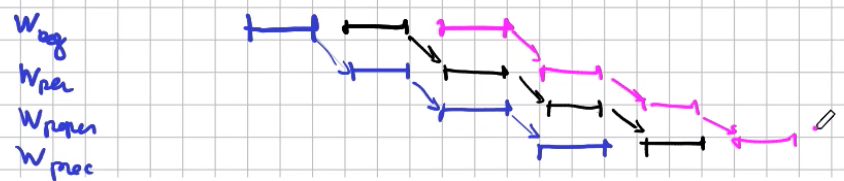
\includegraphics[scale=0.5]{1.png}
\end{center}
So in sequential we have $m\cdot(t_{bag} + t_{pen} + t_{paper} + t_{proc})$, and in parallel per 1 bag we have $t_{bag} + t_{comm} + t_{pen} + t_{comm} + t_{paper} + t_{comm} + t_{proc} + t_{comm}$ with $t_{comm}$ spent passing the bag from one to the other, so total of $m\cdot T_{seq} + m\cdot t_{comm}$. But that's not correct, because we work in parallel: ideally we have a parallelogram of $m\cdot(t_{proc} + t_{comm}$ base, and we require $t_{bag} + t_{pen} + t_{paper} + 3\cdot t_{comm}$ time to get up to speed and "fill the pipeline". But this required time is negligible, and in the end the overall time is given by the base of the parallelogram.
\paragraph{Pipeline} With $m$ tasks and $nw$ stages, with the completion of the stage $i$ required in stage $i+1$. So the output is $f_{nw}(f_{nw-1}(\ldots f_1(x_i)\ldots))$. With $t$ time required for each stage.
\begin{center}
	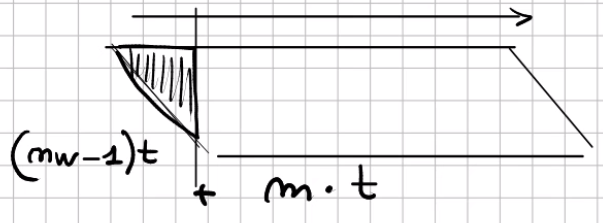
\includegraphics[scale=0.5]{2.png}
\end{center}
We spend $(nw-1)t$ to get the last stage working and $m\cdot t$ time spent by the last stage to complete all the tasks.
$$T_{par}(nw) = (nw-1)\cdot t + m\cdot t$$
$$\hbox{SpeedUp}(nw)=\frac{(nw\cdot t)\cdot m}{(nw-1)\cdot t + m\cdot t}$$
So the higher the $m$ is, the lower is the impact of the time required to get up to speed. So $m >> nw \Rightarrow T_{par}(nw) \simeq m\cdot t$
\paragraph{Throughput} Tasks completed per unit of time.
\section{Measures}
On one side we can have more speed with more resources (computing devices). On the other side we can use more complex applications, with more resources. For example more precise computations, so extra resources not for improving the time but to improve the quality of the computations.\\
Finally, we could aim at computing results with less energy thanks to parallelism. This is a recent perspective on parallelism.\\\\
We've seen the SpeedUp($n$) = $\frac{T_{seq}}{T_{par}(n)}$, where the plot has to lie below the bisection of the cartesian graph.
\subsection{Base Measurements}
\paragraph{Latency $L$} Measure of the wall-clock time between the start and end of the single task.
\paragraph{Service Time $T_s$} It's related to the possibility of executing more tasks. It's the measure of the time between the delivery of two consecutive results, for example between $f(x_i)$ and $f(x_{i+1})$\\
Even if $x_i$ and $x_{i+1}$ arrive at the same time, $f$ would still be computing $f(x_i)$ so it'll start computing $f(x_{i+1})$ when it has finished.
\paragraph{Completion Time $T_c$} The latency related to a number of tasks. $T_c = L\cdot m$ for $x_m,\ldots,x_1$ inputs to a sequential system.\\
With a parallel system, instead, we have $T_c\simeq m\cdot T_s$.
\paragraph{Example} A 3 stage pipeline, with each node being sequential and with latency $L_i$ for node $i$.\\
At $t_0$ the first stage $N_1$ gets the first tasks and computes it in $L_1$, then $N_2$ computes in $L_2$ and $N_3$ computes in $L_3$ so a total of $t_0 + L_1 + L_2 + L_3$.\\
When the pipeline is filled, $T_s$ is dominated by the longest $L_i$, so $T_s = \max\{L_1, L_2, L_3\}$ and $T_c = \sum L_i + (m-1)T_s$\\
If $m$ is large with respect to $n=$ number of stages, the "base of the parallelogram" would be very long, so $m >> n \Leftrightarrow T_c = m\cdot T_s$
\subsection{Derived Measurements}
\paragraph{SpeedUp} $$\hbox{SpeedUp}(n) = \frac{T_{seq}}{T_{par}(n)}$$ Could be latencies, service times\ldots depending on what we want to measure the speedup of.
\paragraph{Scalability} $$\hbox{Scalability}(n)=\frac{T_{par}(1)}{T_{par}(n)}$$
\paragraph{Efficiency} $$\hbox{Efficiency}(n) = \frac{\hbox{Ideal parallel time}(n)}{T_{par}(n)} = \frac{\frac{T_{seq}}{n}}{T_{par}(n)} = \frac{T_{seq}}{n\cdot T_{par}(n)} = \frac{\hbox{SpeedUp}(n)}{n}$$
Measures the tradeoff between what you gain with the speedup and the cost of the speedup.
\paragraph{Throughput} $$\hbox{Throughput} = \frac{1}{T_s}$$
\paragraph{Amdahl Law} Taken the total time of a computation, $T_{seq}$, it can be divided into something that can and something that cannot be computed in parallel (for example, dividing the book is a sequential activity). So we can say that\\$T_{seq} =$ serial fraction + parallel fraction and the \textbf{serial fraction cannot be parallelized}. $f\in[0,1]\:|\:f\cdot T_{seq}$ is the serial fraction.
$$T_{seq} = f\cdot T_{seq} + (1-f)\cdot T_{seq}$$
The parallel fraction can be splitted between the workers, but we would have to compute the serial fraction too. By splitting more and more and more, we have that $$\lim_{n\to\infty} T_{par}(n) = f\cdot T_{seq}$$ $$\hbox{SpeedUp}(n) = \frac{T_{seq}}{f\cdot T_{seq}} = \frac{1}{f}$$
So we have a very low upper bound on the achievable speedup. This is referred to as \textbf{strong scaling}: strong meaning using more resources to get the computation faster.
\paragraph{Gustaffson Law} $$\hbox{SpeedUp}(n) = N - S\cdot(N-1)$$ With $S$ being the serial fraction. This comes from the fact that we're considering a different perspective: Gustaffson assumes that the computation increases with the parallelism, something that's called \textbf{weak scaling}, getting the speedup from using more computational devices, using more data. %TODO rivedere 17/02 inizio parte 2
\paragraph{Cores} In modern computers, we have a main memory (slow), a disk (even slower) and the memory is connected to at least 3 levels of cache. At the bottom we have some cores (4, 8\ldots), each one has its own level 1 cache (usually split in data and instruction cache).\\
With an activity with a working set that fills the cache, in case of strong scaling splitting the computation across cores we process less data per core because the size of the problem is the same.\\
With weak scaling, we assume that the data increases so by using more cores we process the same data on all cores but the data grows so we could have extra overhead because of the working set size.\\
We will have patterns of parallel computation that differentiate in how we process the data.
\paragraph{Application as Graphs} The applications can be seen as graphs of sequential nodes with dependencies.
%TODO
The maximum speedup is the work over the span, because in every case I need to go from the first to the goal node. I take the longest one because at least the longest path must be computed, and all the rest can be done in parallel and I assume to have enough resources to compute the rest in the time of the span.\\
We can use this model %TODO
\section{Technicalities}
\paragraph{Examples}
A simple program that "translates" an ASCII file by transforming lower letters into capital letters. We split the text into $n_{workers}$ parts, we wait for all the threads to finish and then verify the performances.
\\The translator is:
\begin{lstlisting}[style=myC]
#include <string>

char translate_char(char c) {
	if (islower(c))
		return(toupper(c));
	else
		return(tolower(c));
}
\end{lstlisting}
%TODO
\subsection{Threads}
We used to write instructions sequentially. At a given point now we \texttt{fork} another flow of computation: we get two flows that are executed together \textbf{in the same address space}, so the new thread inherits all the memory of the original thread.
\paragraph{Concurrence} \texttt{todo} %TODO
\paragraph{Packaged Threads}
\paragraph{Overheads} % repeatedly fork an join an see what happens, measure mean time of fork-join
All the time spent that is not involved in the sequential execution: time spent organizing the parallel computation, gathering solutions\ldots so there's a tradeoff between the time spent to setup the parallel activity and the time earned because of the parallel execution.\\
What can we do to get rid of the setup time? I can create the threads once and reuse them when needed: \textbf{threadpools}.
\paragraph{Cache Coherence Protocols} Snoopy, or directories of shared data consulted any time I access shared data and propagates the edits.\\
Coherency works at the cache line level!
\subparagraph{In Stencil} Reuse cache coherence protocols for each write.
\subparagraph{False Sharing Problem} We use padding techniques to transform the vector in such way that the original vector has some pad values up to the point where the cache line finishes. This is used in maps.
\subparagraph{Disabling} Sometimes useful to speed up the computations.
\subparagraph{} So we have to take into account that we have to ensure locality as much as possible and be careful of the possibilities of fault sharing problems, like similar iterations in short time.
\paragraph{\texttt{taskset}} To restrict the cores of a process, \texttt{taskset -c 0-3 command} restricts \texttt{command} to the cores 0, 1, 2 and 3.

\section{Patterns}
Computations with particular shapes and semantics that can be understood and implemented depending on the situations, not linked to languages and technicalities. Patterns are a useful concepts, allow programmers to reuse experience of other programmers an not reinventing the wheel.\\
Parallel patterns:
\begin{list}{}{}
	\item Data parallel
	\item Stream parallel
\end{list}
The same patterns can be referred with different names.
\subsection{Data Parallel Patterns}
Parallelism comes from data: we split the data in pieces, compute a set of results that can be combined into a single final result. The book translation examples is a data parallel pattern. What matters is $L$.\\
The general pattern is:
\begin{list}{}{}
	\item Decomposition
	\item Partial results
	\item Recomposition
\end{list}\begin{multicols}{2}
\subparagraph{Map Pattern} Also called applytoall:\begin{list}{}{}
	\item $\forall$ item of the collection
	\item Function $f($item$)$
	\item $\forall$ $f($item$) \rightarrow$ isomorphic collection
\end{list}
\subparagraph{Reduce Pattern} Also called fold:\begin{list}{}{}
	\item $\forall$ item of the collection
	\item $\oplus(x,y)$
	\item $\oplus(\oplus(a,b),\oplus(c,d))$
\end{list}
\end{multicols}
\subparagraph{Stencil Pattern} \begin{list}{}{}
	\item In partially overlapping position, e.g. of a matrix or an image
	\item Function $f($item$)$
	\item $\forall$ $f($item$) \rightarrow$ isomorphic collection
\end{list}
Different kind of problems: overlapping positions will yield the new value, so we have to account for that.
\subparagraph{"Google" mapreduce}
\begin{list}{}{}
	\item $\forall$ items
	\item $f($item$) + \oplus($item$, $item$)$
	\item Item
\end{list}
What I apply to each item is an $f$ that maps to $\langle$key, value$\rangle$ and $\oplus$ applies the sum to each value.\\
For example in a document, $f($word$)=\langle w,1\rangle$ and $\oplus(\langle w_k,v_1\rangle,\langle w_k,v_2\rangle) = \langle w_k, \oplus(v_1,v_2)\rangle$\\
"The lesson given by the professor", $f$ will output $\langle$the, 1$\rangle,\langle$lesson, 1$\rangle$\ldots and $\oplus$ will for example output $\langle$the, 2$\rangle$.\\
We can apply the map function over all the data distributed in various databases, for example.\\
This is \texttt{map(f)} and \texttt{reduce($\oplus$)}, but we want something like \texttt{map(reduce($\oplus$))}. Combining elementary patterns to achieve more complex results. Like two nested \texttt{for}s.\\
So I want building blocks, something that guarantees correctness of implementation that can be used to build upon. For example \texttt{map(function<A(B)>, collection<B>)}\\
So build a bag of tools that we can combine to undertake common situations with good efficiency, speedup, scalability\ldots
\subsection{Stream Parallel Patterns}
Stream of data, flowing in time. In data parallel we process a data collection, while in stream parallel we don't have data appearing all at the same time. So stream as a collection with items appearing at different times. We want to take the single items and try to process in parallel, parallel execution of $f$ over different items of the stream.\\
What matters is $T_S$
\paragraph{Pipeline}
\begin{center}
	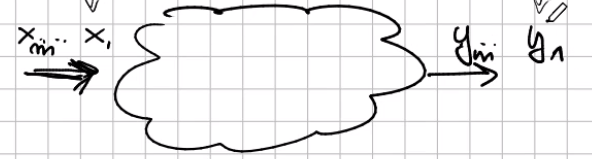
\includegraphics[scale=0.5]{3.png}
\end{center}
Inside the pipeline we have $f_1\rightarrow f_2\rightarrow\ldots\rightarrow f_k$ with each $f_i$ corresponding to a phase, with $f_i$ taking input from $f_{i-1}$.\\
So $x_i\mapsto f_1(x_i)\mapsto f_2(f_1(x_i))\mapsto \ldots$, and the parallelism is in the computation of different phases of different items (much like what we've seen with the CPU fetch-decode-execute pipeline).
\begin{center}
	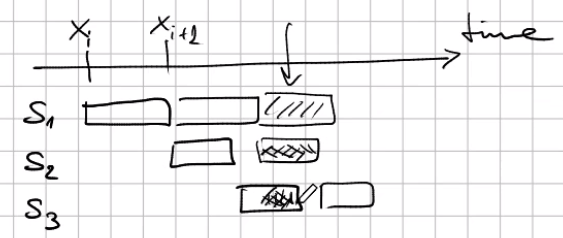
\includegraphics[scale=0.5]{4.png}
\end{center}
\paragraph{Farm}
We have a number $nw$ of instances of the same function $f$ each processing one single item.
\begin{center}
	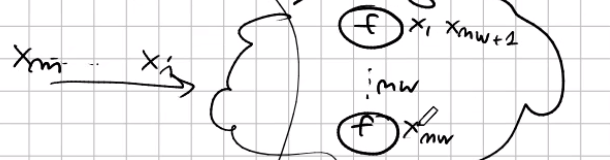
\includegraphics[scale=0.5]{5.png}
\end{center}
We have no interference between computations of $x_i,x_j$ with $i\neq j$, no need for synchronization.
\paragraph{} $T_C \simeq m\cdot T_S$ and $T_S$ in sequential is $\simeq L$ this means that I can try to decrease the latency by decreasing the stages in the pipeline or the workers in a farm.
\paragraph{Two Tier Model} Let's assume a grammar of patterns.\begin{list}{}{}
	\item Pat = Seq(f) $|$ DPP $|$ SPP
	\item DPP = Map(Pat) $|$ Reduce(Pat)
	\item SPP = Farm(Pat) $|$ Pipe(Pat, Pat)
\end{list}
This defines parallel computations and we aim at assuring that this can be done, a way of implementing this. So\begin{list}{}{}
	\item Map(Pipe(Seq(f), Seq(g)))
\end{list}
can be a data parallel computation where on the single item we compute a 2-stages pipeline of $f$ and $g$. But each element of the map is given to a single pipeline, or each pipeline receives a single item, so the stream parallelism is useless.
\begin{list}{}{}
	\item Farm(Map(Seq(f)))
\end{list}
Here we have a stream of items that will be processed by a Farm, each item splitted by Map and processed. This can deliver the result faster and access the next item.\\
So Data parallel with Stream parallel is not very good, Stream parallel with Data parallel is better: \textbf{two tier model}.\\
So we have an initial part of the pattern which is Stream Parallel, the second part is Data Parallel and eventually the last stages (the leafs of the tree) which are sequential.
\paragraph{Parallel Design Patterns}
Also called \textbf{algorithm skeletons}: programming abstraction that model some pattern. The programmer has a framework, libraries, languages and that includes algorithm abstractions.
\subsection{Composing}
These are building blocks, so we can \textbf{compose} them. Let's see how that works and what are the expected performances.
\subsubsection{Pipeline}
We have a number $k$ of stages for $m$ tasks: Pipeline$(s_1,\ldots,s_k)$ meaning that this is a composition yielding $s_k(\ldots s_1(\:)\ldots)$
$$\hbox{Input stream}\longrightarrow s_1\rightarrow\ldots\rightarrow s_k\longrightarrow\hbox{Output stream}$$
With each $\rightarrow$ being a stream $s_i\rightarrow s_{i+1}$ and each $s_i$ taking input from $s_{i-1}$.\\
The latency of the pipeline is the sum of the latencies of the stages $$L(\hbox{Pipeline}(s_1,\ldots,s_k)) = \sum_{i=1}^k L(s_i)$$
We do not consider the time required to pass input to the next stage, $t_{comm}$, which would be based on size, nature of the computation\ldots\\
The steady state is when all the stage are "filled": the longest of the stages will dominate the service time $T_S$
$$T_S(\hbox{Pipeline}(s_1,\ldots,s_k)) = \max_{i=1}^k\{T_S(s_i)\} = \max_{i=1}^k\{L(s_i)\}$$
The completion time is $T_C$
$$T_C(\hbox{Pipeline}(s_1,\ldots,s_k)) = \left(\sum_{i=1}^k L(s_i)\right) + (m-1)\max_{i=1}^k\{L_i\}$$
and when $m >> k$ we can approximate it with
$$T_C = mT_S$$
because the number of tasks required, the "base of the parallelogram", will dominate the number of tasks, the "height of the parallelogram".
\paragraph{Boundary Conditions} We have to take into account the interarrival time $T_A$, time spent to get another item from the input stream, and the interdeparture time $T_D$, the time spent to get another item into the output stream.\\
Let's suppose that $L(s_i) = i$ seconds, so ideally $T_S = k$ seconds: we process 1 item each $k$ seconds. If $T_A > L(s_i)$ we have to wait the second item when I finish processing the first, same thing for the next after the second: the interrarival time looks like an interstage between $s_{i-1}$ and $s_i$.\\
$T_D$ behaves at the same way: we have to wait that $T_D$ finishes before giving it out output, behaving like an interstage.\\
So the previous behavior, analyzed before, happens $\Leftrightarrow T_A<T_S$ and $T_D<T_S$ \textbf{something that we have always to take into account}.
\subsubsection{Farm}
Sometimes we denote as Farm$(s, nw)$, otherwise we omit the number of workers and simply write Farm$(s)$.\\
We assume to know $L_w$ and $T_w$ of the workers. We have some scheduler (\textbf{emitter} $E$) that distributes the items from the input stream to the workers, and a gatherer (\textbf{collector} $C$) that gets the results from the workers and delivers them to the output stream. Those can simply be data structures: queues, for example.
$$L(\hbox{Farm}(s,nw)) = t_E + L_w + t_C$$
This can appear as a pipeline of three stages, where the Emitter produces to the second stage (the workers) which produce to the third stage (the Collector)
$$T_S(\hbox{Farm}(s,nw)) = \max\left\{t_E, \frac{T_w}{nw}, t_C\right\}$$
We assume to have $m$ tasks
$$T_C(\hbox{Farm}(s,nw)) = m\cdot T_S(\hbox{Farm}(s,nw))$$
With boundary conditions
$$T_S=\max\{T_s(\hbox{Farm}()),T_A,T_D\}$$
What if we want to achieve a given performance? Compute a $nw$ suitable to achieve a wanted performance by inverting the very same formulas.\\
With a target $T_S = T_A = 1$s
$$T_S = 1\hbox{s} = \max\left\{t_E, t_C, \frac{10\hbox{s}}{nw}\right\}$$
But $t_E,t_C$ are negligible so $$\frac{10\hbox{s}}{nw} = 1\hbox{s} \Rightarrow nw = 10$$
%TODO riascoltare 2a parte 2/03
\subsubsection{Map} We consider it as made by three phases:
\begin{list}{}{}
	\item Split: divide the collection into sub collections, a \textbf{set of subcollections}
	\item Map: compute the \textbf{set of subresults}
	\item Merge: produce the final \textbf{collection results} (usually in the same shape as the input collection)
\end{list}
With $m$ dimension of the collection and $t_f$ to compute the function of the map $$L(\hbox{Map}) = \frac{m\cdot t_f}{nw} + t_{split} + t_{merge}$$
$t_{split}$ and $t_{merge}$ are non-negligible in distributed architectures, but are negligible in shared-memory architecture.
$$T_S(\hbox{Map}) = L(\hbox{Map})$$
No concept of $T_C$ because the map is applied to a single collection.\\
If I have multiple collections we consider a splitter node as $s_1$, map ($t_f$) as $s_2$ and merger node as $s_3$, giving
$$T_S=\max\{t_{split}, t_{map}, t_{merge}\}$$
$$t_{map} = \frac{m}{nw}t_f$$
\pagebreak
\subsubsection{Reduce}
From a vector we want to output the sum: a scalar from a collection. We split in $t_{split}$, then each of the $nw$ workers applies the function $\oplus$ to its subcollection in $\frac{m}{nw}t_\oplus$ and finally we merge in $nw\cdot t_\oplus$ because we have to compute $\oplus$ over all the $nw$ subresults.
$$L=t_{split} + \left(\frac{m}{nw}-1\right)t_\oplus+(nw-1)t_\oplus$$
$$T_S = L$$
With multiple collections, same argument as before
$$T_S = \max\{\ldots\}$$
But the computation can be organized in a logarithmic tree, too. We would have $\log_2(m)$ phases each with half the activities of the previous phase.\begin{center}
	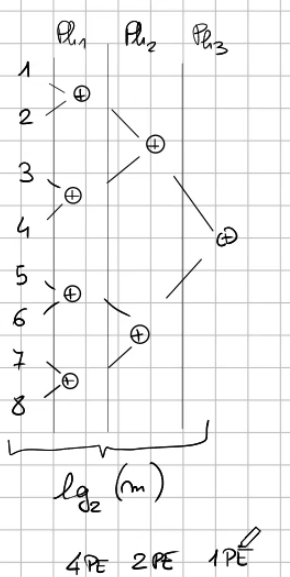
\includegraphics[scale=0.5]{6.png}
\end{center}
But we have efficiency 1 only in the first phase, then half, then one fourth\ldots
$$L=t_{split}+\lceil\log_2 m\rceil t_\oplus$$
provided that $nw \geq \frac{m}{2}$. If we use threads, the split phase is just telling the threads what they have to do, then we merge with a simple loop.
\subsubsection{Stencil}
For example computing the average of three neighbor items in a vector, with necessary boundary conditions.\\
Split phase that produces for example two halves of the vector: when computing the right extreme of the first half, I need to add the first item of the second vector, same with the left extreme of the second half: we have some shared positions. No problem when reading, the problem if we write the shared position. We can use a buffer for the write, using the old values only for reading and swapping the vectors. Or we can use a small buffer to host modified values the neighborhood.
$$L(\hbox{Stencil}) = t_{split} + \frac{m}{nw}t_{stencil} +t_{merge}$$
Where $t_{stencil}$ includes buffer management with the second solution and $t_{merge}$ includes swapping the buffers in the first solution.
\paragraph{Composition} Given a Pipeline($s_1,s_2,s_3$) with $s_i$ sequential, $s_2$ may be data parallel (map), $m$ stream items and each being a vector of $k$ items.
$$L = L_1+L_2+L_3$$
$$T_S=\max\{L_1,L_2,L_3\}$$
$$T_C\simeq m\cdot T_S$$
$s_2$ is sequential but can be turned into a map, takes $L_2$ so I can imagine $t_f \simeq \frac{L_2}{k}$
$$T_S(\hbox{Pipeline}) = \max\left\{L_1,L_3,\frac{L_2}{nw_{map}}\right\}$$
$s_2$ is the slowest stage, we can use a Farm$(s_2, new_{farm})$, but in this case latency stays the same, while using the Map the latency decreases.
\paragraph{Overhead related to memory allocations} New objects are created when instantiating inputs and results, for example. This requires allocating memory in the heap, with corresponding \texttt{malloc}s and \texttt{free}s. So we may need to be smarter, with solutions that work on thread-level memories, small heaps where to allocate objects and releasing when no more needed.
\subparagraph{\texttt{jmalloc} library} Used in BSD systems, FireFox and Facebook among others.\\
It manages \textbf{chunks of memory} called \textbf{arenas}, distributed in a round robin way per thread with each thread using one arena. A metaarena is used a common place.\\
Arenas A1, A2,\ldots, Ak are assigned in round robin to th1, th2\ldots. When some data comes from an arena, and we free that data we free the original arena not the local one. \texttt{jmalloc} has its own API, but other than that it uses the classical API: \texttt{malloc} and \texttt{free}, same as stdlib.\\
Taking a normal program \texttt{a.out}, with \texttt{./a.out p1 \ldots pk} we will go with \texttt{malloc} and \texttt{free} of the stdlib. If we prefix with \texttt{LD\_PRELOAD=libjmalloc.so ./aout p1 \ldots pk} then \texttt{malloc} and \texttt{free} will be loaded from the \texttt{jmalloc} library.
\section{Load Balancing} Giving the same amount of work to all the cores involved. Even if a single thread takes longer than all the other, we wait that it fishes so we have a lot of empty time in the other threads. The efficiency lowers a lot, and poor speedup too.\\
One of the reasons could be that the computation per se is unbalanced.
\subsection{Static Techniques}
Related to the usage of different splitting policies.
\paragraph{Chunk policy} Take the vector and split into adjacent parts
\paragraph{Cyclic policy} First item to first thread, second to second thread\ldots e.g. with two threads: first to th1, second to th2, third to th1, fourth to th2\ldots
\paragraph{Mix} A cyclic distribution of blocks. Split into blocks and assign the first to a thread, the second to the next\ldots following the cyclic policy.
\subsection{Dynamic Techniques}
We can do much more, adapting to the situation giving more things to do to the thread that so far have done less.
\paragraph{Autoscheduling} Threads are not assigned a block/item or a distribution, but each threads \textit{asks} for something to be computed. Some code like \begin{lstlisting}
while (more work to do) {
	ask work
	compute
	deliver result
}
\end{lstlisting}
The threads that gets longer tasks stops asking for more tasks for a while, and more tasks will be executed by the other threads. When tasks are almost finished, it may happen that some thread gets the "last" long task still taking longer than all the other threads. But it's not as impactful as stated before, as it's the worst case.\\
In general, prefetch $k \simeq 2$ or $3$ tasks
\paragraph{Job Stealing} Bunch of tasks, cyclic static assignment. With $nw$ threads and $m$ tasks, each thread gets $\frac{m}{nw}$ tasks. With job stealing, the thread that has finished its tasks and perceives that there's more to compute, steals a task from another thread. Problems: "size" of the steal, synchronize accesses, who to target\ldots the solution is a random policy: threads that finishes their own assigned task steal a random number $\in[0, nw]$ and steal that number of tasks.
\paragraph{Autoscheduling + variable size chunks}

\paragraph{Template Based Implementation} For each pattern (pipe, farm, map, stencil\ldots) we have templates:\begin{list}{}{}
	\item for each target architecture (multicore, cloud\ldots)
	\item activity graph
	\item performance modelling, also a way to have an idea of what we can achieve in terms of perfomance
\end{list}
Let's analyze a template for a pipeline on a shared memory multicore machine (\texttt{template(pipeline, SMmulticore)}):
$$\longrightarrow\hbox{thread}\rightarrow\hbox{thread}\rightarrow\ldots\rightarrow\hbox{thread}\longrightarrow$$
With the $\rightarrow$ being communication channels (queues). Modelling the speedup$(m)\simeq m$ with $m$ being the number of stages, so a linear speedup, if and only if $\max\{t_i\}\simeq t_j$ so the times of each stage are more or less the same.\\\\
But we can have another template
$$x_m\ldots x_2\:x_1\longrightarrow\hbox{queue}$$
Where in the queue we put "\texttt{compute} $f$ \texttt{over} $x_i$" as $\langle f,x_i\rangle$ for each $i$. Each worker gets $\langle f,x\rangle$ and puts in the queue $\langle g, f(x)\rangle$. For $\langle g,x\rangle$ returns $\langle h,g(x)\rangle$ and for $\langle h,x\rangle$ returns $\langle$ end$,h(x)\rangle$.\\
So the queue will have different types of tasks: the input tasks are assigned to $f$ but the intermediate tasks are assigned to $g$ or $h$: it's a pipeline. Of course, the end tasks means outputting on the output queue.\\
A problem: the queue is a bottleneck. We can use some techniques: set of queues, local queues\ldots Also the ordering, but i can keep the index $i$ for each stage and use it at the end to keep in a buffer and output in the correct order.\\
With modeling provided sufficient $T_A$, the speedup can be proportional to $nw$ and not $m$.\\\\
Another template is a round-robin scheduler that assigns to some workers that deliver results to sorter with respect to the input order. The scheduler gives $\langle i, x_i\rangle$ and the output is $h(g(f(x_i)))$ ordered on $i$. Pipeline. Uses $nw+2$ concurrent activities, with a queue for each worker plus a queue for the sorter. With $T_A$ low, we have speedup circa $nw$.\\\\
Changing architecture, from shared memory multicore to a clustered workstation. I can use any template ported to a cluster. For example
$$\hbox{workstation}_1\rightarrow_{\hbox{TCP/IP}}\hbox{workstation}_2\ldots$$
The speedup is circa the number of stages. But we can also have a number of workers in each workstation, with a scheduler and a merger per each. A kind of composed template, the third inside the stages of the first.
$$T_S\simeq\frac{\max\{T_i\}_{nw}}{nw}$$
The overhead is in the scheduling and merging parts of each stage. The scheduling is necessary, but in the ordering part we sort data on the input order, but we can do that just at the end of the last stage.
\paragraph{Macro Data Flow Implementation} With Data Flow we denote the operations where the order of computations are dictated by the flow of data encountered by the program counter.\\
So we have nodes that are composed of $\langle$ operator, variables, output$\langle$. For example, $$(a+b)\cdot(c-d)$$ can be represented as 
\begin{center}
	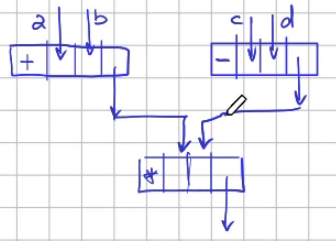
\includegraphics[scale=0.5]{7.png}
\end{center}
We have tokens on the inputs, that represent when data are available. When all data is available, the node becomes "fireable". This technique can be used to implement parallel patterns, Macro because instead of considering operations as nodes with functions an input/output nodes we consider macros with full portions of code instead of primitive functions.\\
Let's consider a program \texttt{main.cpp} that uses some pattern internally from a pattern library. First step: from a pattern tree we compile the MDF (Macro Data Flow graph). We have a graph repository and a pool of executors: anytime I have some input data I create a copy of the graph in the repository with the tokens that represent the data.\begin{center}
	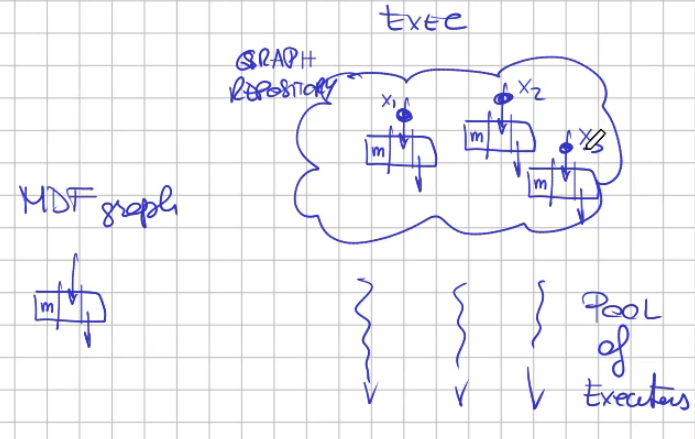
\includegraphics[scale=0.5]{8.png}
\end{center}
Each executor executes a loop where they get a fireable instruction, compute and deliver the output tokens.
\paragraph{Compiler} From the Pattern Tree it outputs the MDF graph.
\begin{list}{}{}
	\item Compile(Pipe($f,g$)) $\rightarrow$ $\langle f,$ in, A$\rangle$, $\langle g,$ A, out$\rangle$
	\item Compile(Seq($f$)) $\rightarrow$ $\langle f,$ in, out$\rangle$
	\item Compile(Farm($f$)) $\rightarrow$ Compile($f$) for each instance of input
	\item Compile(Map($f$)) $\rightarrow$ Compile($f$) for each element of the input collection
	\begin{center}
		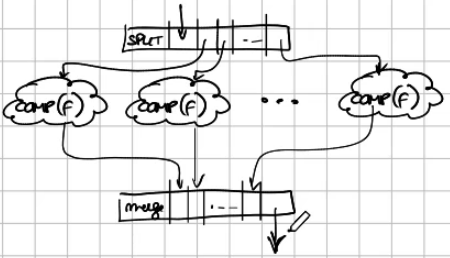
\includegraphics[scale=0.5]{9.png}
	\end{center}
	\item Compile(Reduce($f$)) $\rightarrow$ \begin{center}
		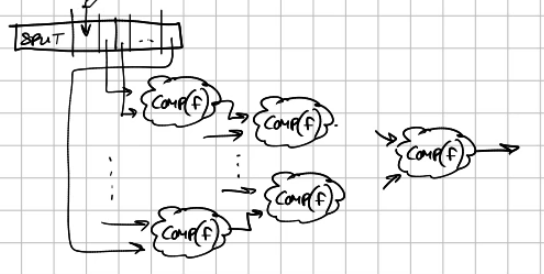
\includegraphics[scale=0.5]{10.png}
	\end{center}
\end{list}
Each one of the graphs has one input token and one output token, mandatory to be able to compose the graph. The Farm parallelism disappears %TODO
and third %TODO
\paragraph{Problems}\begin{list}{}{}
	\item Contention over repository
	\item Token delivery
	\item Maintain the list of fireable instructions
	\item Reordering on the out stream
\end{list}
\paragraph{Refactoring Rules}
The grammar used to write our program is:
\begin{center}
	Pat = Seq() $|$ Pipe(Pat$_1$, Pat$_2$) $|$ Comp(Pat$_1$, Pat$_2$) $|$ Farm(Pat, $nw$) $|$ Map(Pat) $|$ Reduce(Map)\\
	Prog $\Rightarrow$ Pat : $x$\\
	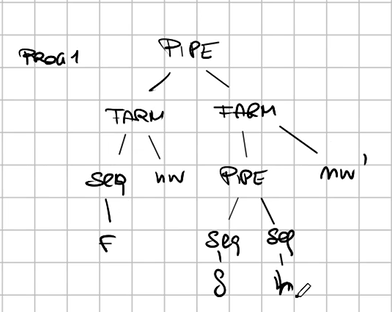
\includegraphics[scale=0.5]{12.png}
\end{center}
Whit \textbf{functional semantics} we mean \textbf{what is computed}. \textbf{Non-functional semantics} refers to \textbf{how} the result \textbf{is computed}.\\
So refactoring rules describe the equivalences in the \textbf{functional semantics}. So different performance, parallelism degrees\ldots\\
Some examples:
\begin{list}{}{}
	\item Farm($x, n$) $\equiv$ Farm($x, m$) with $n\neq m$
	\item Pipe($x, y$) $\equiv$ Comp($x, y$)
	\item Pipe(Farm($x, \_$), Farm($y, \_$)) $\equiv$ Farm(Pipe($x, y$) \_)
\end{list}
How to figure out the better ones? We will consider a small set of rules:
\begin{list}{}{}
	\item \textbf{Pipe introduction/elimination}: Comp($x,y$) $\equiv$ Pipe($x,y$)
	\item \textbf{Farm introduction/elimination}: $x \equiv$ Farm$(x)$
	\item \textbf{Map fusion}: Map(Comp($x,y$)) $\equiv$ Comp(Map($x,y$))
	\item \textbf{Pardegree change}: Farm($x, n$) $\equiv$ Farm($x, m$) with $n\neq m$
\end{list}
The idea is to write a program (so a tree $T_0$) and apply the rules (via a tool) getting $T_1,T_2,\ldots$ all functionally equivalent to $T_0$. Usually the goal is a low $T_{S_i}$. We take the produced trees, mapping each to its $T_S$ and reducing to $\min$ to get the minimum $T_{S_k}$.\\
But maybe we compute worse trees. I can do another thing: taking $T_0$ trying to find the path in the possible trees. I apply rules and measure the metric (in this example, $T_S$). Then I don't go exploring all the subtrees, applying all applicable rules, but I just go one level down and pick the best one each time. We follow a path that always gives a better (or equivalent) performing solution. But this is \textbf{not possible}.
%TODO why, 2nd part 22/03
With a lot of approximations and details ignored, I can figure out the best parallel architecture.
\paragraph{Normal Form} Speaking of stream parallel computations. Optimizes the service time $T_S$ (more precisely, the throughput).\\
We can derive the normal form from every pattern tree, only with stream parallel patterns\begin{enumerate}
	\item \textbf{Get the frontier}, set of all the sequential leaves in the tree, \textbf{left to right}.
	\item Comp(frontier), so sequential composition in the order they appear.
	\item Farm(Comp(frontier))
\end{enumerate}
This process always aims at optimizing the parallel computation. Unless there are some particular reasons. We take the whole set of things to compute an put them together (1 and 2), meaning creating a chunk of code that do the work: \textbf{increase the grain of the computation}.\\
This optimizes the service time taking also into account resources.
\paragraph{Performance Models} Used to evaluate or to optimize.\\
\textbf{Evaluate} meaning that, having a tree, we evaluate a metric (e.g. $T_S$) visiting the tree from the leaves. For each leaf we're interested in the sequential time ($T_S = L$ for the sequential nodes). The we go up one step visiting the parents: we have the parameters of the subtree and can compute $T_S$ of the node given its subtrees. We can repeat until the root.\\\
The visit of a tree is also a pattern, so if I take that pattern (visiting a tree from the leaves upward) passing the tree as a parameter I can get a number of different \textbf{visitors}: $T_S$ in this case is a visitor. For example, for Visitor(\# resources) we would visit the tree in the same way but using a different formula for computing the contribution of each node.\\
\textbf{Optimize} the parameters, for example the parallel degrees of the stages. In \texttt{rplsh} we used \texttt{optimize main with max resources}. How it's implemented? We take the tree, with Pipe in the root, same as before. We turn the tree with the $nw$ figured out, but we have a certain number of resources. For example we want to shrink the number of resources to match the number of cores.
\paragraph{RPLShell} \begin{center}
	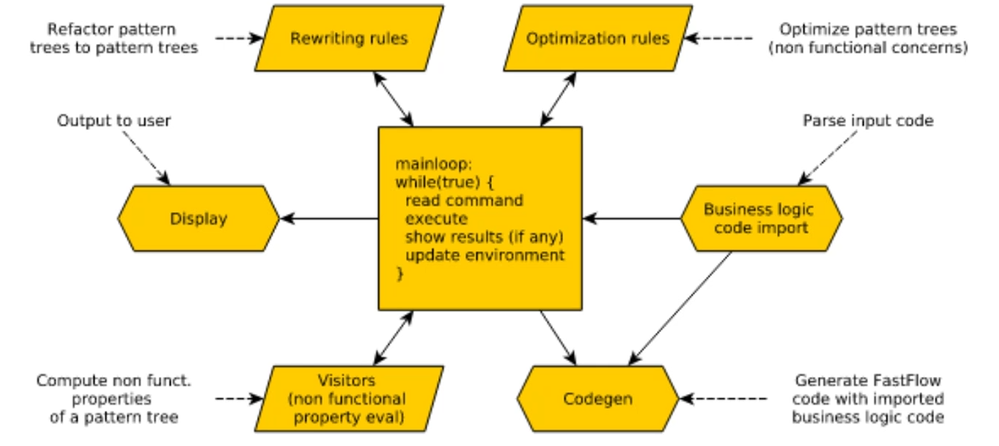
\includegraphics[scale=0.5]{13.png}
\end{center}
\begin{list}{}{}
	\item \textbf{Rewriting Rules} are the set of factoring rules.\\
	For example, we have the facts that allow me to rewrite a given tree $t$ as Farm($t$) or Pipe($t_1,t_2$) as Comp($t_1,t_2$).
	\item \textbf{Optimiziation Rules} the set of rules that for example transform a Farm(Farm($w$)) into Farm($w$) (because two farms linked are bad for performance), known as farmfarmopt, or the farmopt that is used when we have Farm($w$) with a certain $T_S$ of the $w$ and a certain $T_S$ target of the farm in order to set the $nw$ of the farm to $\frac{T_S}{T_{S,w}}$.
	\item \textbf{Visitors} the elements that visit the tree upwards.
\end{list}
\paragraph{Autonomic Management of Non Functional Features} In long running computations.\\
For example the classical variations in network load between night and day. Autonomic because %TODO
Born from industrial processes management, changing behaviors of the systems. Different architectures of the controller:
\begin{list}{}{}
	\item \textbf{MAPE Loop} (Monitor, Analyze, Plan, Execute loop)\\
	Execute activities via actuators, and the system has a set of actuator objects that can be invoked to change the behavior of the system (for instance changing $nw$). The system has sensors, too, that provide data to the monitor part.
\end{list}
We have to devise a strategy to be used. E.g.: if $T_A$ drops, most likely I could just increase $nw$ and viceversa if $T_A$ increases I can drop $nw$. Being more clever: let's suppose that $T_A$ goes from $T_{A_{\max}}$ to $T_{A_{\min}}$ in a $\sin$ fashion, when I'm in the minimum I could take time in taking a decision to increase $nw$ while $T_A$ is already increasing. Same for the maximum, I could spend time making the decision and always arriving late. So our strategy can be update: I can observe the changes and avoid situations of alternating opposite changes (in the example, the adding and taking away workers constantly).\\\\
To implement these strategies, I need \textbf{sensors} and \textbf{actuators}.\\
We need to observe the interarrival time $T_A$. Also need a data structure to observe the changes, by doesn't require sensors. These sensors would be in the emitter thread.\\
We need to increase or decrease $nw$, so the actuators must be able to achieve that. To add a worker, e.g. a thread, we need to know the queue for that worker, the collector\ldots so the emitter sounds like a good place.\\\\
This is implemented in the \textbf{control program} of our manager. Very crude \texttt{if (condition) do actuator;}.
\paragraph{ECA Rules} Set of \textbf{Event, Condition, Action} rules implemented in a rule system (e.g. \texttt{jboss}).\begin{list}{}{}
	\item \textbf{Event}: \textbf{triggering action}, e.g. $T_A$ change.\\
	Not the event per se to be taken into account.
	\item \textbf{Condition}: \textbf{predicates} on monitored values, internal state and events, that state whenever this particular rule has to be fired or not.
	\item \textbf{Action}: \textbf{set of actions} on the system or the state that must be \textbf{executed after some triggering event when the condition holds true}.
\end{list}
\subparagraph{Example}
\begin{center}
	\begin{tabular}{c | c c c}
	& \textbf{Event} & \textbf{Condition} & \textbf{Action}\\
	\hline
	$R_1$ & Change $T_A$ & \makecell{Less than the\\previous one} & Adding a worker\\\\
	$R_2$ & Change $T_A$ & \makecell{More than the\\previous one} & Removing a worker\\\\
	$R_3$ & Change $T_A$ & \makecell{Less than the\\previous one AND\\$nw$ just decreased} & \texttt{nop}, update $T_A$\\\\
	$R_4$ & Change $T_A$ & \makecell{More than the\\previous one AND\\$nw$ just increased} & \texttt{nop}, update $T_A$
	\end{tabular}
\end{center}
\paragraph{Contracts}\begin{enumerate} %TODO
	\item Propagate the "contract" top-down and try to implement it "best-effort"
	\item Manage to keep contracts satisfied 
\end{enumerate}
We're taking into accounts performance, but often power consumption is more important. These are both non-functional features. If we take into account both, we could implement a manager for each. But the managers may take decision that contrast with each other. A solution is to build a single manager that takes into account both features, into a single MAPE loop. But this requires that both knowledge are in a single place, bad for the separation of concerns. Another solution is to have two managers, one for each feature, each with its MAPE loop, and the two can communicate: the plan phase inform each other in the hope to have authorization for a change that the execute part needs, if we don't get the authorization we go for a \texttt{nop}.
\begin{center}
	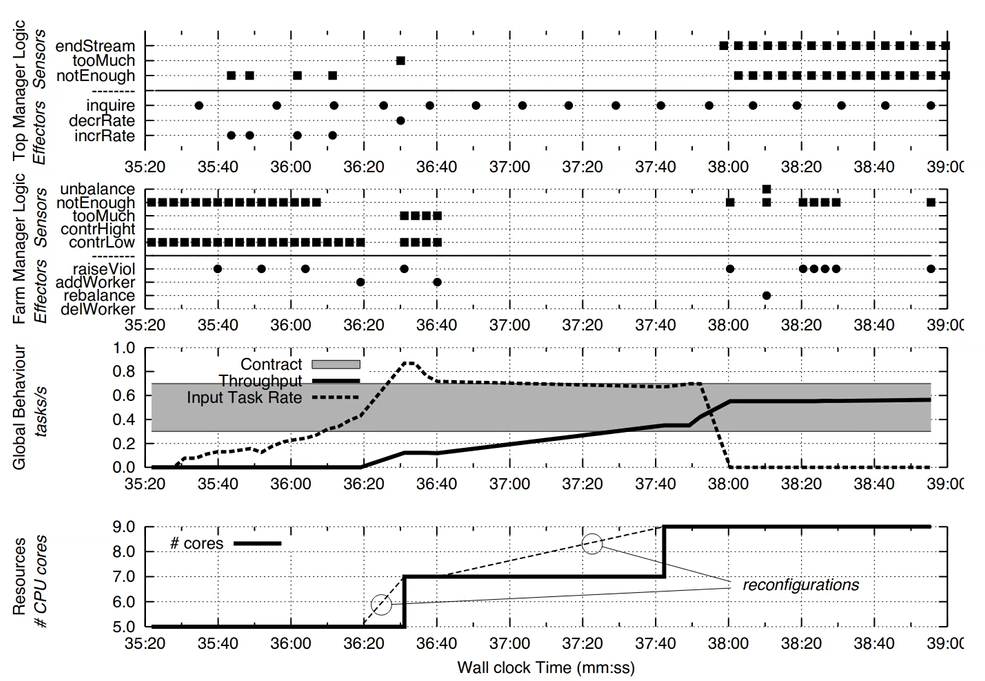
\includegraphics[scale=0.5]{15.png}
\end{center}
\section{Vectorization}
Very old technique. %TODO
Given $x, y, z$ as vectors of $x_i, y_i, z_i$ from $0$ to $n-1$ and $\forall\:i\in[0,n-1]\:\:z_i=f(x_i,y_i)$, implemented e.g. as a \texttt{for}. If the computation $f(x_i, y_i)$ is indepdendent of the other loop iterations (that is, $x_i$ is independent from all other $x_j, j\neq i$) then this is easily parallelized. A classical example is matrix multiplication: $$\forall\:i\:\:\forall\:j\:\:\forall\:k\:\:c_{ij} = a_{ik}\cdot b_{kj}$$
2 steps: we need to have zeroes in the first positions and %TODO
We have ways to load/store vectors to %TODO

Hardware designed specifically, vector processors. Registers that can be seen as vectors of tot bits numbers: 256 bits vector registers seen as 4 64 bits numbers, or 8 32 bits numbers and so on. With special commands, for example \texttt{VADD.I32 R1, R2, R3} meaning R1 = R2 + R3 with I32 meaning 32 bit numbers with I index.
\paragraph{Conditions} In \texttt{g++} we can explicitly ask with \texttt{-03 -ftree-vectorize} and with \texttt{-fopt-info-vec-[missed/all]} ask what cannot be vectorize.\\
The conditions are:
\begin{list}{}{}
	\item Need to know the number of iterations.\\
	\texttt{for} is ok, \texttt{while(c$<$k)} sometimes cannot be vectorized
	\item Cannot call external code in the loop body, functions or libraries.
	\item No conditional code.\\
	It'd require compiling two paths, so complicates things.
	\item No overlapping pointers.\\
	
\end{list}
\paragraph{\texttt{\#pragma}} Indications to the compiler\\
\texttt{\#pragma GCC ivdep} tells the compiler whatever it thinks of the loop, to consider it as independent iterations.\\
\texttt{\#pragma GCC unroll n} tells the compiler that the following loop should be unrolled \texttt{n} times. Useful for short loops.\\\\
So vectorization very useful for mathematical operations, such as differential equations. Requires to take a bit of care in the core to be able to vectorize. If we don't convince the compiler, we can use the \texttt{pragma}.\\
If we vectorize Farm($f,nw$), the speedup with the vectorized $f$ with respect to the non-vectorized $f$ is smaller. Because the vectorized code in general is faster, so non-vectorized Speedup($nw$) $Z$ Vectorized Speedup($nw$).\\
But vectorization can radically change the $T_S$ of the stages of a Farm, for instance, and introduce waiting times for workers. You don't change the sequential fraction, just the non-sequential fraction.
\paragraph{Libraries} Libraries include operations used often, e.g. \texttt{Blas} (basic linear algebra system) or \texttt{Lapack} or \texttt{NKL}.\\
For instance \texttt{blas} provides \texttt{gemm} for very optimized matrix multiplications.\\
Use libraries because they are very optimized, exploiting all the possible optimizations.
\paragraph{GRPPI} C++ library that implements common parallel patterns, using standard threads or other backends (e.g. omp, tdd or fastflow). The backend is only modeled by the \texttt{execution} parameter.
\section{OpenMP}
\paragraph{MPi} Directed to clusters and workstations, multicores
\paragraph{CDA/OpenCL} For GPU
\paragraph{OpenMP} Parallel for, targets shared memory multicores (and GPU/FPGA). Very dated, since 1997 the version 1.0: no GPU, even multicores were not very popular.\\
At the beginning very simple API that provided launching threads in parallel and something related to the parallel for. Each version improved on that, introducing: tasks, target accelerators, depend clauses on tasks (to tell that a task must be executed only after the completion of another task), memory management, task reduction (among values of different tasks), task affinity\ldots\\
When we speak about shared memory multicores, we speak of some situation where in the board we have more than one sockets with multicore in each socket.
\paragraph{Concepts}\begin{list}{}{}
	\item \textbf{Directives}, which OpenMP is based on. Directives, in C/C++ environment, are kind of pragmas which can be understood as portions of compiler
	\item OpenMP is \textbf{compiler-based}
	
\end{list}
As pros:
\begin{list}{}{}
	\item Few lines of code are required to run parallel code, opposed to writing all the logic by oneself
	\item Keep sequential code, means we can perform functional debugging and then adding parallel pragmas
\end{list}
As main con we need to rewrite the compiler, not entirely (such as the parser), but everything related to the usage of the pragmas must be generated at compile time.\\
E.g. the map seen in the GRPPI library is written at higher level but in the library, doesn't touch the compiler.\\\\
We have something used to \textbf{set up parallel activities} and something different used to \textbf{organize the parallel computation} using the parallel activities available.
\paragraph{\texttt{\#pragma omp parallel}} This must be placed before a statement, it tells the compiler that the following block must be executed in $nw$ copies (threads) if and only if $nw$ is the number of resources/cores of the current machine.\\
Most directives have clauses used to specify parameters. E.g. \texttt{num\_threads(nw)} tells to use the variable $nw$ instead of the predefined one (the number of cores).
\begin{lstlisting}[style=myC]
#include <iostream>
#include <omp.h>

using namespace std;
int main(int argc, char** argv) {
	int nw = 1;
	if (argc != 1)
		nw = atoi(argv[1]);
	#pragma omp parallel num_threads(nw) // clause
	{
		auto id = omp_get_thread_num();
		cout << "Ciao from id " << id << endl;
	}
	return(0);
}
\end{lstlisting}
\paragraph{\texttt{\#pragma omp single}} Specifies that the following statement/block is to be executed by just a single thread.
\begin{lstlisting}[style=myC]
#include <iostream>
#include <omp.h>

using namespace std;
int main(int argc, char** argv) {
	int nw = 1;
	if (argc != 1) {
		nw = atoi(argv[1]);
		#pragma omp parallel num_threads(nw)
		{
			#pragma single // this will be executed by a single thread, just one enters the following line, use a block for more lines
			cout << "Id " << omp_get_thread_num() << " of " << omp_get_num_threads() endl;
		}
	} else {
		#pragma omp parallel
		{
			auto id = omp_get_thread_num();
			cout << "Id " << id << " of " << omp_get_num_threads() endl;
		}
	}
	return(0);
}
\end{lstlisting}
\paragraph{\texttt{\#pragma omp critical}} To execute the next code in mutual exclusion.
\paragraph{To use OpenMP} Compile with flag \texttt{-openmp}.\\
The \texttt{a.out} compiled, when executed, uses the linked library which provides several things including a lock/mutex machanism. So instead of the \texttt{\#pragma omp critical} we can use \texttt{\#pragma omp parallel} and then just the lock/unlock:
\begin{lstlisting}[style=myC]
omp_lock_t lock;
omp_init_lock(&lock);
#pragma omp parallel
{
	// code
	omp_set_lock(&lock);
	// mutex code
	omp_unset_lock(&lock);
	// code
}
\end{lstlisting}
With the code/unlock declared with respect to the OpenMP library.
\paragraph{Different code for different threads} We can do something like
\begin{lstlisting}[style=myC]
#pragma omp parallel num_threads(2)
{
	if (omp_get_thread_num() == 0) {
		// code for thread 1
	} else {
		// code for thread 2
	}
}
\end{lstlisting}
This is \textbf{SPMD} code: single program multiple data.
\paragraph{Sections directive}
\begin{list}{}{}
	\item \texttt{\#pragma omp sections}: identifies a command which is filled by other \texttt{section} directives, each executed possibly in parallel
	\item \texttt{\#pragma omp section}
\end{list}
Example
\begin{lstlisting}[style=myC]
#pragma omp sections
{
	#pragma omp section
	{
		//code 1
	}
	#pragma omp section
	{
		//code 2
	}
}
\end{lstlisting}
All the \texttt{section} may happen in parallel, how much is defined and can be inherited by other statements. For example I can have a \texttt{\#pragma omp parallel} before the \texttt{\#pragma omp sections}, giving the threads explained before (the number of cores as default, or as specified by \texttt{num\_threads(nw)}.
\paragraph{Variables} In most directives you can append clauses that specifies the behavior of variables.\\
For example in parallel pragmas you can append the clauses\begin{list}{}{}
	\item\texttt{private(x)} (non initialized local copy local to each thread)
	\item\texttt{firstprivate(x, y)} (get a local copy initialized from previous value)
	\item\texttt{shared(y, z)} (inherit value from the global environment)
	\item\texttt{lastprivate(x)} (this one legal only in sections, not in parallel, local copy then last \texttt{section} copied to global environment, take care last one means in syntactic-fashion, the last syntactic section updating the variables copies to global environment)
\end{list}
\paragraph{\texttt{\#pragma omp for}} Most famous and used.\\
The default behavior is that the iterations, e.g. from $i=0$ to $i=n-1$, are made into $nw$ chunks given each to a thread. Obviously we need independent iterations. There are others scheduling policies, specified with clauses appended to the \texttt{\#pragma omp for}:
\begin{list}{}{}
	\item \texttt{static} the default one, with the option of specifying \texttt{chunksize(m)} specifying the number of items in each chunk, so $\frac{n-1}{m}$ chunks of $m$ items, given to the threads in a round-robin fashion
	\item \texttt{dynamic} where the threads ask for new chunks when they have finished, chunks are assigned on demand. Same of the static for other things
	\item \texttt{guided} use a number of chunks smaller and smaller: large chunks in the first part of the array, then smaller chunks, then smaller and so on. Intended to be used for unbalanced computations: at the beginning we assign large chunks to each thread, but the threads may finish at different times and get smaller chunks to accomodate for load unbalancing
	\item \texttt{auto} everything decided by the compiler
	\item \texttt{runtime} keyword which inherits the scheduling policy from an environment variable which has to be defined before 
\end{list}
You also have other clauses
\begin{list}{}{}
	\item \texttt{nowait}, removes the implicit barrier to wait all the threads, present in the parallel pragma
	\item \texttt{reduction([+,*,and,or], x)}
\end{list}
\paragraph{\texttt{\#pragma omp task}} Kind of async, suggestion that if there are unusued threads use to compute the task otherwise it's sequential code.\\
Can define taskgroups to execute in parallel and wait with the implicit barrier at the end.\\
You can append \texttt{tied} or \texttt{untied}: with the first anytime you assign/reassign the execution of this task then it would be on the same thread.\\
The taskloop provides something similar to a map, or a pragma for, but subjecting to the rules of the tasks: could be executed in parallel given enough resources ecc.
\paragraph{Example} Sum of a vector with a reduce(+), base case being a vector of length 1 so return the value v[0]. Otherwise the recursive case is a vector of $n$ positions: compute the half and split in v[0,$\frac{n}{2}$] and v[$\frac{n}{2},n$] recur. So we need a task for the left half, a task for the right part, checking not to be in the base case.
\begin{lstlisting}[style=myC]
int sum (int* restricted v, int start, int end) {
	auto size = end - start;
	auto mid = size/2;
	int x, y; //shared for the subtasks, sum from left and right
	
	if (size == 1) return v[start]; //base case
	
	#pragma omp task shared(x) //to share the result with this "main" thread
	{
		x = sum(v, start, start+mid);
	}
	#pragma omp task shared(y) //same as befor
	{
		y = sum(v, end-mid, end);
	}
	#pragma omp taskwait //wait for the termination of the tasks, a "barrier"
	//now both tasks have finished, we have both x and y
	return x+y;
}

int main(int argc, char** argv) {
	#pragma omp parallel num_threads(nw) //or from the CLI "export OMP_NUM_THREADS=nw"
	//...
	#pragma omp single //single or master
	sum(v, 0, n-1);
}
\end{lstlisting}
\paragraph{Timing routines} Also present.
\end{document}